\documentclass[12pt]{article}
\usepackage[utf8]{inputenc}
\usepackage{amsmath}
\usepackage{amsfonts}
\usepackage{amssymb}
\usepackage{geometry}
\usepackage{booktabs}
\usepackage{tcolorbox}
\usepackage{tikz}
\geometry{a4paper, margin=1in}

\usetikzlibrary{arrows.meta, positioning, calc, decorations.pathreplacing}

\title{Arithmetic Coding and Range Coding: A Detailed Tutorial}
\author{}
\date{}

\begin{document}

\maketitle

\section{Arithmetic Coding and Range Coding: A Detailed Tutorial}

\subsection{Introduction}

Entropy coding is the final stage in many compression systems.
Instead of assigning fixed codewords to symbols (like Huffman coding),
\textbf{Arithmetic Coding} and \textbf{Range Coding} represent the entire
message as a single number inside the unit interval $[0,1)$.
This allows code lengths to approach the theoretical entropy limit.

\begin{tcolorbox}[colback=blue!3,colframe=blue!40!black,title=Key Idea]
Arithmetic coding does not assign codes to symbols individually.
Instead, it assigns a code to the entire \textit{sequence} by repeatedly shrinking an interval.
The more probable the message, the larger the final interval and the fewer bits needed.
\end{tcolorbox}

We now explain arithmetic coding in detail, followed by a complete worked
example, a comparison with range coding, and finally the same example solved
using range coding.

\subsection{Arithmetic Coding: Theory and Algorithm}

Arithmetic coding encodes a message by repeatedly narrowing an interval in $[0,1)$.
Each symbol reduces the interval based on its probability.

\begin{tcolorbox}[colback=blue!3,colframe=blue!40!black,title=Algorithm: Arithmetic Coding Encoding]
\textbf{Step 0: Initialization} \\
Set $\text{low} = 0$ and $\text{high} = 1$.

\vspace{2mm}
\textbf{Step 1: Compute cumulative frequencies} \\
Given an alphabet $\{s_1, s_2, \dots, s_k\}$ with probabilities $p(s_i)$, compute:
\[
C(s_1) = 0, \qquad C(s_i) = \sum_{j < i} p(s_j) \text{ for } i = 2, 3, \dots, k
\]

\vspace{2mm}
\textbf{Step 2: For each symbol in the message to be encoded} \\
For each symbol $s$ (taken in order from the message), perform:
\begin{align*}
\text{range} &= \text{high} - \text{low} \\
\text{high} &= \text{low} + \text{range} \times (C(s) + p(s)) \\
\text{low} &= \text{low} + \text{range} \times C(s)
\end{align*}

\vspace{2mm}
\textbf{Step 3: Generate the final code} \\
After encoding all symbols, any number $x$ in the interval $[\text{low}, \text{high})$ represents the entire message. Typically, we output:
\[
\text{code} = \frac{\text{low} + \text{high}}{2} \quad \text{(the midpoint of the final interval)}
\]
\end{tcolorbox}

\subsection{Example: Arithmetic Coding Step-by-Step}

Consider the alphabet $\{A,B,C\}$ with frequencies:

\[
f(A)=5,\qquad f(B)=3,\qquad f(C)=2,\qquad \text{Total}=10.
\]

Thus probabilities:

\[
p(A)=0.5,\qquad p(B)=0.3,\qquad p(C)=0.2.
\]

We want to encode the message:

\[
\text{MESSAGE} = \texttt{BAC}
\]

\subsubsection*{Step 0: Initialization}
\[
\text{low} = 0,\qquad \text{high} = 1
\]

\subsubsection*{Step 1: Compute cumulative frequencies}
The cumulative frequencies define the sub-interval boundaries and are sorted in alphabetical order:

\[
C(A) = 0,\qquad C(B) = p(A) = 0.5,\qquad C(C) = p(A) + p(B) = 0.8
\]

\subsubsection*{Step 2: Encode each symbol in the message}

\textbf{Symbol 1: B}

\begin{align*}
\text{range} &= \text{high} - \text{low} = 1 - 0 = 1 \\
\text{high} &= \text{low} + \text{range} \times (C(B) + p(B)) = 0 + 1 \times (0.5 + 0.3) = 0.8 \\
\text{low} &= \text{low} + \text{range} \times C(B) = 0 + 1 \times 0.5 = 0.5
\end{align*}

Interval after encoding B: $[0.5,\; 0.8)$

\vspace{2mm}
\textbf{Symbol 2: A}

\begin{align*}
\text{range} &= \text{high} - \text{low} = 0.8 - 0.5 = 0.3 \\
\text{high} &= \text{low} + \text{range} \times (C(A) + p(A)) = 0.5 + 0.3 \times (0 + 0.5) = 0.5 + 0.15 = 0.65 \\
\text{low} &= \text{low} + \text{range} \times C(A) = 0.5 + 0.3 \times 0 = 0.5
\end{align*}

Interval after encoding A: $[0.5,\; 0.65)$

\vspace{2mm}
\textbf{Symbol 3: C}

\begin{align*}
\text{range} &= \text{high} - \text{low} = 0.65 - 0.5 = 0.15 \\
\text{high} &= \text{low} + \text{range} \times (C(C) + p(C)) = 0.5 + 0.15 \times (0.8 + 0.2) = 0.5 + 0.15 \times 1.0 = 0.65 \\
\text{low} &= \text{low} + \text{range} \times C(C) = 0.5 + 0.15 \times 0.8 = 0.5 + 0.12 = 0.62
\end{align*}

Final interval after encoding all symbols: $[0.62,\; 0.65)$

\subsubsection*{Step 3: Generate the final code}

Any number in $[0.62, 0.65)$ encodes the message \texttt{BAC}. We choose the midpoint:

\[
\text{code} = \frac{0.62 + 0.65}{2} = 0.635
\]

This is the arithmetic-coded representation of \texttt{BAC}. In practice, we would output this number in binary form.

\begin{figure}[h!]
\centering
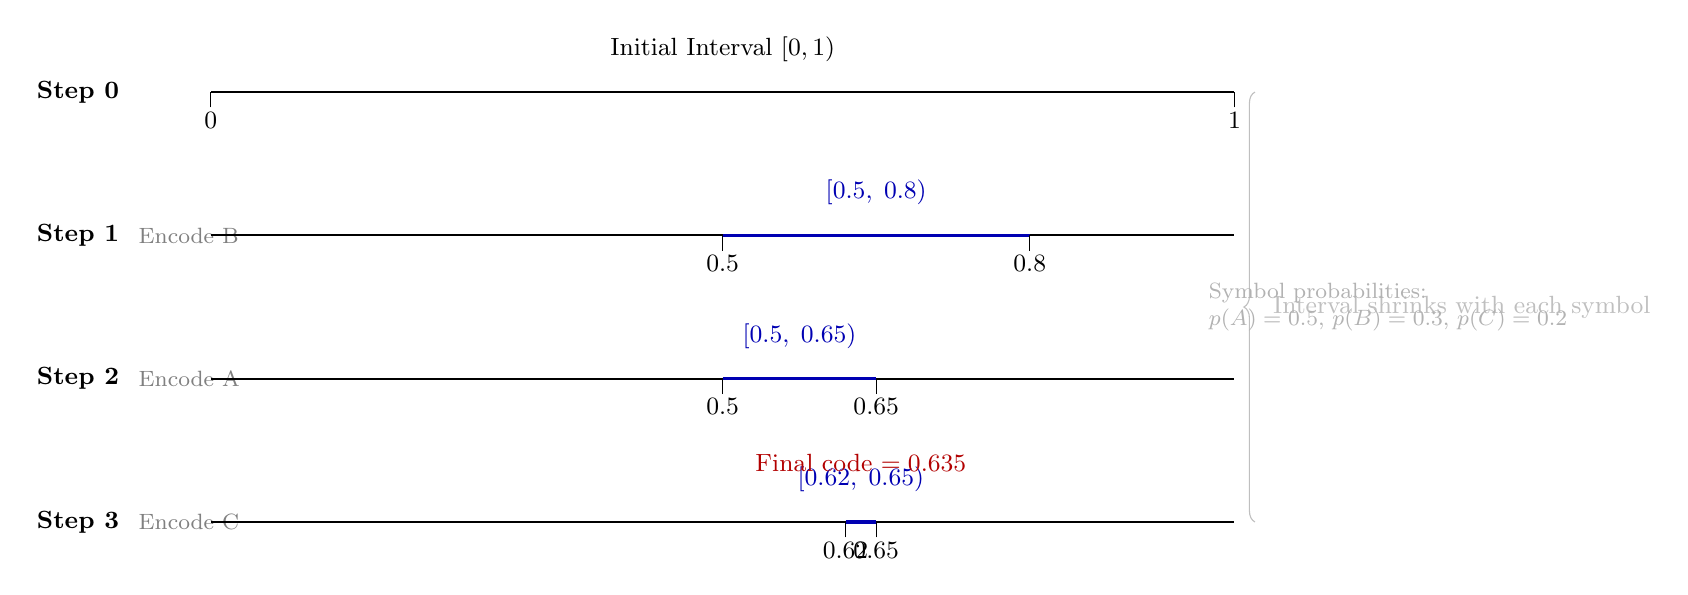
\begin{tikzpicture}[scale=1.3, 
    every node/.style={font=\small},
    interval/.style={thick},
    selected/.style={very thick, blue!70!black},
    annotation/.style={font=\footnotesize, text=gray}
]

% Initial interval
\node[anchor=east] at (-0.8,0) {\textbf{Step 0}};
\draw[interval] (0,0) -- (10,0);
\draw[annotation] (0,-0.15) -- (0,0);
\draw[annotation] (10,-0.15) -- (10,0);
\node[below] at (0,-0.1) {$0$};
\node[below] at (10,-0.1) {$1$};
\node[above] at (5,0.2) {Initial Interval $[0,1)$};

% Step 1: Encode B → [0.5, 0.8)
\node[anchor=east] at (-0.8,-1.4) {\textbf{Step 1}};
\node[annotation, right] at (-0.8,-1.4) {Encode B};
\draw[interval] (0,-1.4) -- (10,-1.4);
\draw[selected] (5,-1.4) -- (8,-1.4);
\draw[annotation] (5,-1.55) -- (5,-1.4);
\draw[annotation] (8,-1.55) -- (8,-1.4);
\node[below] at (5,-1.5) {$0.5$};
\node[below] at (8,-1.5) {$0.8$};
\node[above, blue!70!black] at (6.5,-1.2) {$[0.5,\;0.8)$};

% Step 2: Encode A → [0.5, 0.65)
\node[anchor=east] at (-0.8,-2.8) {\textbf{Step 2}};
\node[annotation, right] at (-0.8,-2.8) {Encode A};
\draw[interval] (0,-2.8) -- (10,-2.8);
\draw[selected] (5,-2.8) -- (6.5,-2.8);
\draw[annotation] (5,-2.95) -- (5,-2.8);
\draw[annotation] (6.5,-2.95) -- (6.5,-2.8);
\node[below] at (5,-2.9) {$0.5$};
\node[below] at (6.5,-2.9) {$0.65$};
\node[above, blue!70!black] at (5.75,-2.6) {$[0.5,\;0.65)$};

% Step 3: Encode C → [0.62, 0.65)
\node[anchor=east] at (-0.8,-4.2) {\textbf{Step 3}};
\node[annotation, right] at (-0.8,-4.2) {Encode C};
\draw[interval] (0,-4.2) -- (10,-4.2);
\draw[selected] (6.2,-4.2) -- (6.5,-4.2);
\draw[annotation] (6.2,-4.35) -- (6.2,-4.2);
\draw[annotation] (6.5,-4.35) -- (6.5,-4.2);
\node[below] at (6.2,-4.3) {$0.62$};
\node[below] at (6.5,-4.3) {$0.65$};
\node[above, blue!70!black] at (6.35,-4.0) {$[0.62,\;0.65)$};
\node[above, red!70!black] at (6.35,-3.8) {Final code $=0.635$};

% Add a visual guide showing the shrinking process
\draw[decorate, decoration={brace, amplitude=4pt, mirror}, gray!50] 
    (10.2,0) -- (10.2,-4.2) node[midway, right, xshift=3pt] 
    {Interval shrinks with each symbol};

% Add probability annotation
\node[annotation, text=gray!60, align=left] at (11.5,-2.1) 
    {Symbol probabilities:\\ 
    $p(A)=0.5$, $p(B)=0.3$, $p(C)=0.2$};

\end{tikzpicture}
\caption{Arithmetic Coding Interval Refinement for Message \texttt{BAC}. 
Each step selects a sub-interval based on the symbol being encoded. 
The final code $0.635$ is the midpoint of the final interval $[0.62,0.65)$.}
\label{fig:arithmetic}
\end{figure}


\subsection{Why People Prefer Range Coding}

Arithmetic coding is theoretically elegant but has practical implementation challenges:

\begin{itemize}
    \item \textbf{Arbitrary precision requirement:} As encoding progresses, the interval becomes very small. To represent the final interval precisely, we need high-precision arithmetic. For long messages, this requires arbitrary-precision numbers or specialized libraries.
    
    \item \textbf{Incremental output complexity:} In practice, we don't want to wait until the entire message is encoded before outputting bits. Instead, we output bits incrementally as they become fixed. This process—often called \textit{normalization} or \textit{bit-stuffing}—requires careful handling of carry propagation.
    
    \item \textbf{Computational cost:} Multiplication and division operations at each step are more expensive than the integer operations used in range coding.
    
    \item \textbf{Historical patent issues:} Arithmetic coding was subject to patents for many years, discouraging its use in some applications (though this is no longer an issue today).
\end{itemize}

\begin{tcolorbox}[colback=yellow!5,colframe=orange!70!black,title=Normalization in Arithmetic Coding]
Unlike floating-point numbers that can underflow to zero, the interval in arithmetic coding never underflows—it simply becomes very small. The term \textit{normalization} in arithmetic coding refers to the process of \textbf{outputting bits incrementally} as they become known, not to preventing precision loss. 

For example, after encoding the first few symbols, the interval $[0.5, 0.8)$ tells us that the first bit of the output will be \texttt{1} (since the entire interval lies in the top half of $[0,1)$). We can output that bit immediately and double the interval to continue encoding.

If we are content to store the entire final fraction (like $0.635$) without incremental output, no normalization is needed. However, for long messages, storing the full precision fraction becomes impractical, which is why incremental output is used in real implementations.
\end{tcolorbox}

\textbf{Range Coding} addresses these challenges:
\begin{itemize}
    \item Uses fixed-precision integer arithmetic (e.g., 32-bit or 64-bit integers)
    \item Handles incremental output naturally through renormalization
    \item Uses only integer operations (division, multiplication, shifts)
    \item Faster on most hardware architectures
\end{itemize}

Range coding is simply a \textbf{reparameterization of arithmetic coding} designed for efficient implementation.

\textbf{Range Coding} solves these problems while producing the same outputs
and remaining mathematically identical.

Range coding is simply a \textbf{reparameterization of arithmetic coding}
designed for efficiency.

\subsection{Range Coding: Theory and Algorithm}

Range coding works on integers rather than real-number intervals. The fundamental insight is that we can scale the $[0,1)$ interval to a large integer range, e.g., $[0, 2^{32})$. All operations then become integer arithmetic.

\begin{tcolorbox}[colback=blue!3,colframe=blue!40!black,title=Algorithm: Range Coding Encoding]
\textbf{Step 0: Initialization} \\
Set $\text{low} = 0$ and $\text{range} = R$ (a large integer, typically $2^{32}$).

\vspace{2mm}
\textbf{Step 1: Compute cumulative frequencies} \\
Given an alphabet $\{s_1, s_2, \dots, s_k\}$ with frequencies $f(s_i)$ and total frequency $\text{total} = \sum_i f(s_i)$, compute:
\[
C(s_1) = 0, \qquad C(s_i) = \sum_{j < i} f(s_j) \text{ for } i = 2, 3, \dots, k
\]

\vspace{2mm}
\textbf{Step 2: For each symbol in the message to be encoded} \\
For each symbol $s$ (taken in order from the message), perform:
\begin{align*}
\text{unit} &= \text{range} / \text{total} \quad \text{(integer division)} \\
\text{low} &= \text{low} + \text{unit} \times C(s) \\
\text{range} &= \text{unit} \times f(s)
\end{align*}

\vspace{2mm}
\textbf{Step 3: Renormalization (incremental output)} \\
When $\text{range}$ falls below a threshold (e.g., $2^{24}$), the most significant bits of $\text{low}$ are stable and can be output. We:
\begin{itemize}
    \item Output the top byte (most significant 8 bits) of $\text{low}$
    \item Shift $\text{low}$ and $\text{range}$ left by 8 bits
\end{itemize}
This is analogous to outputting bits incrementally in arithmetic coding.

\vspace{2mm}
\textbf{Step 4: Generate the final code} \\
After encoding all symbols, output the remaining bytes of $\text{low}$ to complete the compressed representation.
\end{tcolorbox}

The key difference from arithmetic coding is that range coding uses:
\begin{itemize}
    \item Fixed-precision integers instead of arbitrary-precision real numbers
    \item Integer division and multiplication instead of floating-point operations
    \item A renormalization process that outputs bytes (groups of bits) rather than individual bits
\end{itemize}

\subsection{Range Coding Example (Same Message)}

We now encode the same message \texttt{BAC} using integer range coding. We'll use a smaller initial range of $R = 2^{16} = 65536$ for simplicity in our calculations. The process is identical with $2^{32}$.

\subsubsection*{Step 0: Initialization}
\[
\text{low} = 0,\qquad \text{range} = 65536
\]

\subsubsection*{Step 1: Compute cumulative frequencies}
\[
f(A)=5,\quad f(B)=3,\quad f(C)=2,\quad \text{total}=10
\]
\[
C(A)=0,\quad C(B)=5,\quad C(C)=8
\]

\subsubsection*{Step 2: Encode each symbol in the message}

\textbf{Symbol 1: B}

\begin{align*}
\text{unit} &= \frac{65536}{10} = 6553 \quad \text{(integer division truncates)} \\
\text{low} &= 0 + 6553 \times 5 = 32765 \\
\text{range} &= 6553 \times 3 = 19659
\end{align*}

\textbf{Real-number equivalent:} $\left[\frac{32765}{65536}, \frac{32765+19659}{65536}\right) \approx [0.5000, 0.8000)$

\vspace{2mm}
\textbf{Symbol 2: A}

\begin{align*}
\text{unit} &= \frac{19659}{10} = 1965 \\
\text{low} &= 32765 + 1965 \times 0 = 32765 \\
\text{range} &= 1965 \times 5 = 9825
\end{align*}

\textbf{Real-number equivalent:} $\left[\frac{32765}{65536}, \frac{32765+9825}{65536}\right) \approx [0.5000, 0.6500)$

\vspace{2mm}
\textbf{Symbol 3: C}

\begin{align*}
\text{unit} &= \frac{9825}{10} = 982 \\
\text{low} &= 32765 + 982 \times 8 = 32765 + 7856 = 40621 \\
\text{range} &= 982 \times 2 = 1964
\end{align*}

\textbf{Real-number equivalent:} $\left[\frac{40621}{65536}, \frac{40621+1964}{65536}\right) \approx [0.6198, 0.6498)$

\subsubsection*{Step 3: Renormalization (skipped for simplicity)}

In a real implementation, we would renormalize when range becomes too small.

\subsubsection*{Step 4: Generate the final code}

The final integer interval is $[\text{low}, \text{low}+\text{range}) = [40621, 42585)$.
Any integer in this range encodes the message. We output the value $40621$ as our compressed representation.

%%%%
\begin{figure}[h!]
\centering
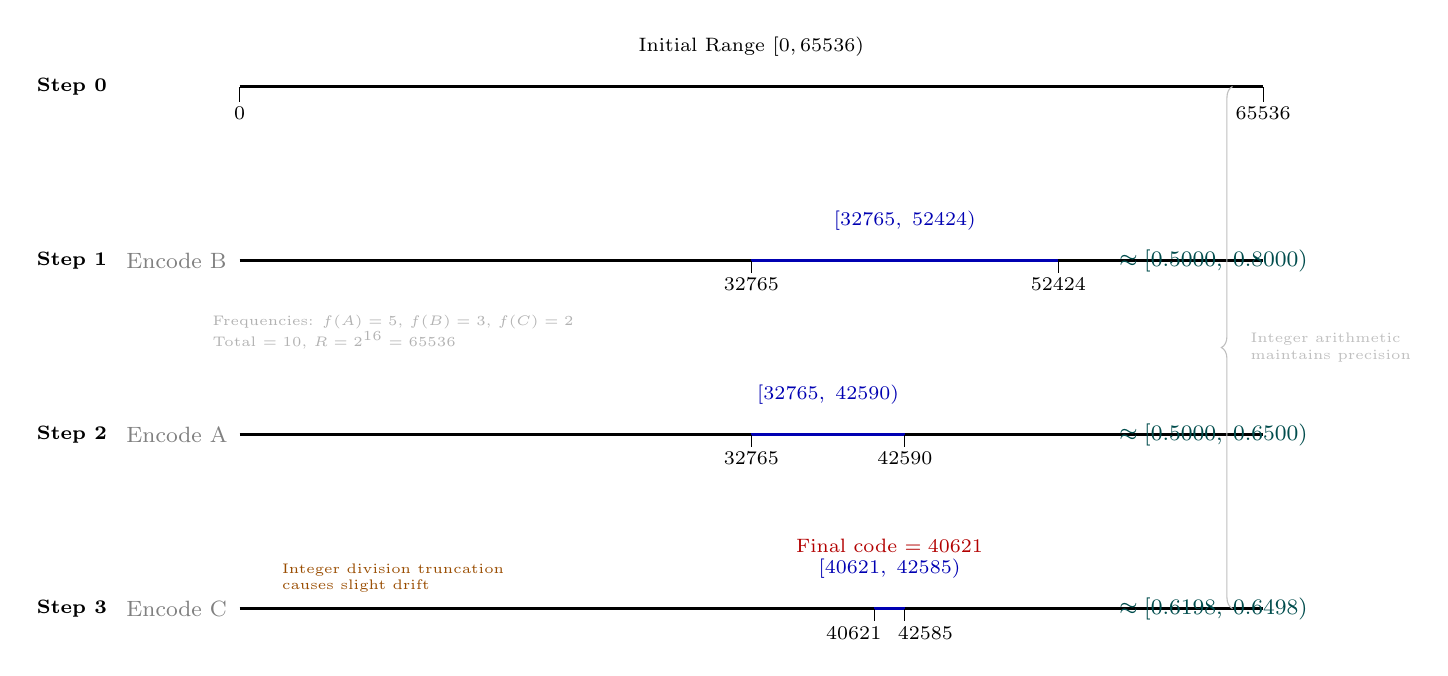
\begin{tikzpicture}[scale=1.3,
    every node/.style={font=\scriptsize},
    interval/.style={thick},
    selected/.style={very thick, blue!70!black},
    annotation/.style={font=\footnotesize, text=gray}
]

% Moderate spacing
\def\stepheight{1.7}

% Initial interval
\node[anchor=east] at (-1.2,0) {\textbf{Step 0}};
\draw[interval] (0,0) -- (10,0);
\draw[annotation] (0,-0.15) -- (0,0);
\draw[annotation] (10,-0.15) -- (10,0);
\node[below] at (0,-0.1) {$0$};
\node[below] at (10,-0.1) {$65536$};
\node[above] at (5,0.2) {Initial Range $[0,65536)$};

% Step 1: Encode B → [32765, 52424)
\node[anchor=east] at (-1.2,-\stepheight) {\textbf{Step 1}};
\node[annotation, right] at (-1.2,-\stepheight) {Encode B};
\draw[interval] (0,-\stepheight) -- (10,-\stepheight);
\draw[selected] (5,-\stepheight) -- (8,-\stepheight);
\draw[annotation] (5,-\stepheight-0.12) -- (5,-\stepheight);
\draw[annotation] (8,-\stepheight-0.12) -- (8,-\stepheight);
\node[below] at (5,-\stepheight-0.08) {$32765$};
\node[below] at (8,-\stepheight-0.08) {$52424$};
\node[above, blue!70!black] at (6.5,-\stepheight+0.2) {$[32765,\;52424)$};

% Real-number equivalent placed to the RIGHT
\node[annotation, text=teal!60!black, anchor=west] at (8.5,-\stepheight) 
    {$\approx [0.5000,\;0.8000)$};

% Step 2: Encode A → [32765, 42590)
\node[anchor=east] at (-1.2,-2*\stepheight) {\textbf{Step 2}};
\node[annotation, right] at (-1.2,-2*\stepheight) {Encode A};
\draw[interval] (0,-2*\stepheight) -- (10,-2*\stepheight);
\draw[selected] (5,-2*\stepheight) -- (6.5,-2*\stepheight);
\draw[annotation] (5,-2*\stepheight-0.12) -- (5,-2*\stepheight);
\draw[annotation] (6.5,-2*\stepheight-0.12) -- (6.5,-2*\stepheight);
\node[below] at (5,-2*\stepheight-0.08) {$32765$};
\node[below] at (6.5,-2*\stepheight-0.08) {$42590$};
\node[above, blue!70!black] at (5.75,-2*\stepheight+0.2) {$[32765,\;42590)$};

% Real-number equivalent placed to the RIGHT
\node[annotation, text=teal!60!black, anchor=west] at (8.5,-2*\stepheight) 
    {$\approx [0.5000,\;0.6500)$};

% Step 3: Encode C → [40621, 42585)
\node[anchor=east] at (-1.2,-3*\stepheight) {\textbf{Step 3}};
\node[annotation, right] at (-1.2,-3*\stepheight) {Encode C};
\draw[interval] (0,-3*\stepheight) -- (10,-3*\stepheight);
\draw[selected] (6.2,-3*\stepheight) -- (6.5,-3*\stepheight);
\draw[annotation] (6.2,-3*\stepheight-0.12) -- (6.2,-3*\stepheight);
\draw[annotation] (6.5,-3*\stepheight-0.12) -- (6.5,-3*\stepheight);
\node[below] at (6.0,-3*\stepheight-0.08) {$40621$};
\node[below] at (6.7,-3*\stepheight-0.08) {$42585$};
\node[above, blue!70!black] at (6.35,-3*\stepheight+0.2) {$[40621,\;42585)$};
\node[above, red!70!black] at (6.35,-3*\stepheight+0.45) {Final code $=40621$};

% Real-number equivalent placed to the RIGHT
\node[annotation, text=teal!60!black, anchor=west] at (8.5,-3*\stepheight) 
    {$\approx [0.6198,\;0.6498)$};

% Add brace showing integer nature
\draw[decorate, decoration={brace, amplitude=4pt, mirror}, gray!50] 
    (9.7,0) -- (9.7,-3*\stepheight) node[midway, right, xshift=3pt, align=left, font=\tiny] 
    {Integer arithmetic\\ maintains precision};

% Add frequency annotation
\node[annotation, text=gray!60, align=left, font=\tiny] at (1.5,-2.4) 
    {Frequencies: $f(A)=5$, $f(B)=3$, $f(C)=2$\\ 
    Total $=10$, $R=2^{16}=65536$};

% Add note about truncation
\node[annotation, text=orange!60!black, font=\tiny, align=left]  at (1.5,-4.8) 
    {Integer division truncation\\ causes slight drift};

\end{tikzpicture}
\caption{Range Coding Integer-Interval Refinement for Message \texttt{BAC}. Real-number equivalents are shown to the right.}
\label{fig:range}
\end{figure}
\subsection{Direct Comparison: Arithmetic vs. Range Coding}

The following table summarizes the parallel between the two methods:

\begin{center}
\begin{tabular}{l | l | l}
\toprule
\textbf{Concept} & \textbf{Arithmetic Coding} & \textbf{Range Coding} \\
\midrule
Representation & Real numbers in $[0,1)$ & Integers in $[0, R)$ \\ \hline
Initial state & $\text{low}=0$, $\text{high}=1$ & $\text{low}=0$, $\text{range}=R$ \\
Unit size & $\text{range} = \text{high}-\text{low}$ & $\text{unit} = \text{range} / \text{total}$ \\
Low update & $\text{low} + \text{range} \times C(s)$ & $\text{low} + \text{unit} \times C(s)$ \\
Range update & $\text{range} \times p(s)$ & $\text{unit} \times f(s)$ \\
Precision handling & Floating-point normalization & Integer renormalization \\
Final code & Midpoint of final interval & Integer from final interval \\
\bottomrule
\end{tabular}
\end{center}

\subsection{Summary}

\begin{itemize}
    \item Arithmetic coding uses real-number intervals and is mathematically elegant.
    \item Range coding uses integer intervals but produces the same final interval.
    \item Range coding is faster in practice because it avoids floating-point arithmetic and uses only integer operations.
    \item Both achieve compression close to the theoretical entropy limit.
    \item The two methods are mathematically equivalent; range coding is simply an integer-based implementation of arithmetic coding.
\end{itemize}

\subsection{Exercises for Students}

\begin{enumerate}
    \item Encode the message \texttt{CAB} using arithmetic coding with the same probabilities. Show each step.
    \item Encode the same message \texttt{CAB} using range coding with $R=65536$ and compare the final intervals.
    \item Explain why range coding is more suitable for hardware implementation than arithmetic coding.
    \item What would happen if we used a smaller initial range, such as $R=1000$, for range coding? How would it affect compression quality?
    \item Write pseudocode for an arithmetic coding encoder and a range coding encoder. Identify the key differences.
    \item Using the figures provided, explain how the interval refinement process differs between arithmetic coding and range coding.
    \item Why is the update order (first high, then low) important in arithmetic coding?
    \item What is the purpose of renormalization in range coding? Why wasn't it needed in our simple example?
\end{enumerate}

\end{document}
